\documentclass{standalone}
\usepackage{tikz}
\usetikzlibrary{patterns, positioning}


\begin{document}
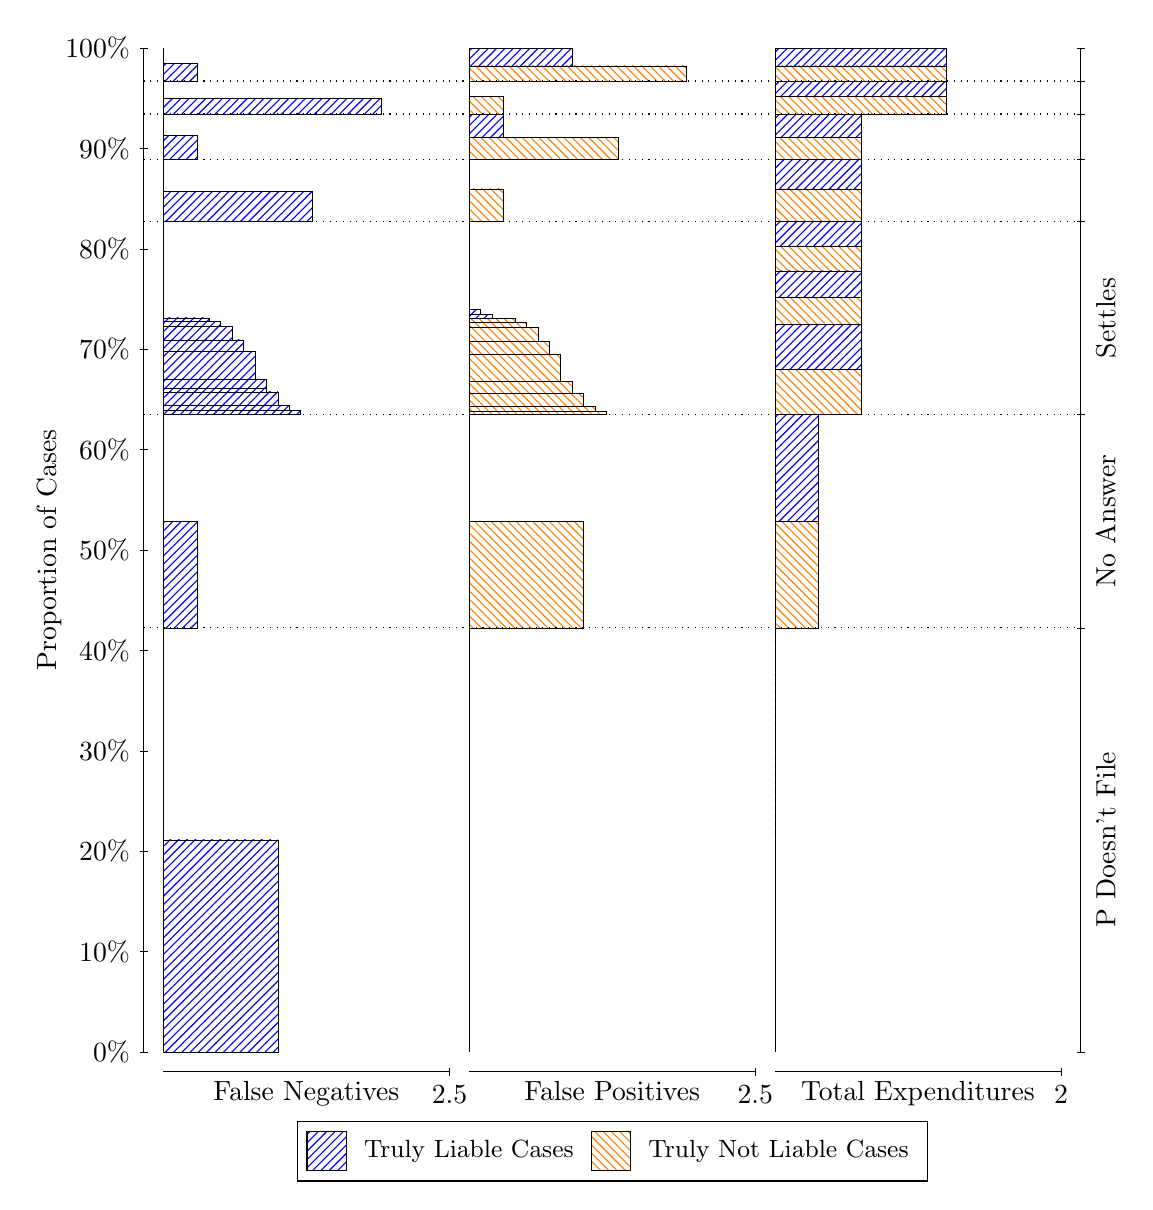
\begin{tikzpicture}
\draw[black, very thin] (1.5,1.75) -- (1.5,14.5);
\node[rotate=90, text=black, anchor=center] at (0.3, 8.125) {Proportion of Cases};
\draw[black, very thin] (1.45,1.75) -- (1.55,1.75);
\node[text=black, anchor=east] at (1.45, 1.75) {0\%};
\draw[black, very thin] (1.45,3.025) -- (1.55,3.025);
\node[text=black, anchor=east] at (1.45, 3.025) {10\%};
\draw[black, very thin] (1.45,4.3) -- (1.55,4.3);
\node[text=black, anchor=east] at (1.45, 4.3) {20\%};
\draw[black, very thin] (1.45,5.575) -- (1.55,5.575);
\node[text=black, anchor=east] at (1.45, 5.575) {30\%};
\draw[black, very thin] (1.45,6.85) -- (1.55,6.85);
\node[text=black, anchor=east] at (1.45, 6.85) {40\%};
\draw[black, very thin] (1.45,8.125) -- (1.55,8.125);
\node[text=black, anchor=east] at (1.45, 8.125) {50\%};
\draw[black, very thin] (1.45,9.4) -- (1.55,9.4);
\node[text=black, anchor=east] at (1.45, 9.4) {60\%};
\draw[black, very thin] (1.45,10.675) -- (1.55,10.675);
\node[text=black, anchor=east] at (1.45, 10.675) {70\%};
\draw[black, very thin] (1.45,11.95) -- (1.55,11.95);
\node[text=black, anchor=east] at (1.45, 11.95) {80\%};
\draw[black, very thin] (1.45,13.225) -- (1.55,13.225);
\node[text=black, anchor=east] at (1.45, 13.225) {90\%};
\draw[black, very thin] (1.45,14.5) -- (1.55,14.5);
\node[text=black, anchor=east] at (1.45, 14.5) {100\%};

\draw[black, very thin] (13.4,1.75) -- (13.4,14.5);
\draw[black, very thin] (13.35,1.75) -- (13.45,1.75);
\node[anchor=west] at (13.35, 1.75) {};
\draw[black, very thin] (13.35,7.1369) -- (13.45,7.1369);
\node[anchor=west] at (13.35, 7.1369) {};
\draw[black, very thin] (13.35,9.8424) -- (13.45,9.8424);
\node[anchor=west] at (13.35, 9.8424) {};
\draw[black, very thin] (13.35,12.298) -- (13.45,12.298);
\node[anchor=west] at (13.35, 12.298) {};
\draw[black, very thin] (13.35,13.088) -- (13.45,13.088);
\node[anchor=west] at (13.35, 13.088) {};
\draw[black, very thin] (13.35,13.662) -- (13.45,13.662);
\node[anchor=west] at (13.35, 13.662) {};
\draw[black, very thin] (13.35,14.081) -- (13.45,14.081);
\node[anchor=west] at (13.35, 14.081) {};
\draw[black, very thin] (13.35,14.5) -- (13.45,14.5);
\node[anchor=west] at (13.35, 14.5) {};

\draw[black, very thin, pattern color=blue, pattern=north east lines] (1.75,1.75) rectangle (3.2033,4.4434);
\draw[black, very thin, pattern color=orange, pattern=north west lines] (1.75,4.4434) rectangle (1.75,7.1369);
\draw[black, very thin, pattern color=blue, pattern=north east lines] (1.75,7.1369) rectangle (2.186,8.4896);
\draw[black, very thin, pattern color=orange, pattern=north west lines] (1.75,8.4896) rectangle (1.75,9.8424);
\draw[black, very thin, pattern color=blue, pattern=north east lines] (1.75,9.8424) rectangle (3.494,9.897);
\draw[black, very thin, pattern color=blue, pattern=north east lines] (1.75,9.897) rectangle (3.3487,9.9578);
\draw[black, very thin, pattern color=blue, pattern=north east lines] (1.75,9.9578) rectangle (3.2033,10.132);
\draw[black, very thin, pattern color=blue, pattern=north east lines] (1.75,10.132) rectangle (3.058,10.177);
\draw[black, very thin, pattern color=blue, pattern=north east lines] (1.75,10.177) rectangle (3.058,10.296);
\draw[black, very thin, pattern color=blue, pattern=north east lines] (1.75,10.296) rectangle (2.9127,10.643);
\draw[black, very thin, pattern color=blue, pattern=north east lines] (1.75,10.643) rectangle (2.7673,10.793);
\draw[black, very thin, pattern color=blue, pattern=north east lines] (1.75,10.793) rectangle (2.622,10.96);
\draw[black, very thin, pattern color=blue, pattern=north east lines] (1.75,10.96) rectangle (2.4767,11.024);
\draw[black, very thin, pattern color=blue, pattern=north east lines] (1.75,11.024) rectangle (2.3313,11.072);
\draw[black, very thin, pattern color=orange, pattern=north west lines] (1.75,11.072) rectangle (1.75,12.298);
\draw[black, very thin, pattern color=blue, pattern=north east lines] (1.75,12.298) rectangle (3.6393,12.676);
\draw[black, very thin, pattern color=orange, pattern=north west lines] (1.75,12.676) rectangle (1.75,13.088);
\draw[black, very thin, pattern color=blue, pattern=north east lines] (1.75,13.088) rectangle (2.186,13.388);
\draw[black, very thin, pattern color=orange, pattern=north west lines] (1.75,13.388) rectangle (1.75,13.662);
\draw[black, very thin, pattern color=blue, pattern=north east lines] (1.75,13.662) rectangle (4.5113,13.856);
\draw[black, very thin, pattern color=orange, pattern=north west lines] (1.75,13.856) rectangle (1.75,14.081);
\draw[black, very thin, pattern color=blue, pattern=north east lines] (1.75,14.081) rectangle (2.186,14.309);
\draw[black, very thin, pattern color=orange, pattern=north west lines] (1.75,14.309) rectangle (1.75,14.5);
\draw[black, very thin, pattern color=orange, pattern=north west lines] (5.6333,1.75) rectangle (5.6333,4.4435);
\draw[black, very thin, pattern color=blue, pattern=north east lines] (5.6333,4.4435) rectangle (5.6333,7.1369);
\draw[black, very thin, pattern color=orange, pattern=north west lines] (5.6333,7.1369) rectangle (7.0867,8.4896);
\draw[black, very thin, pattern color=blue, pattern=north east lines] (5.6333,8.4896) rectangle (5.6333,9.8424);
\draw[black, very thin, pattern color=orange, pattern=north west lines] (5.6333,9.8424) rectangle (7.3773,9.888);
\draw[black, very thin, pattern color=orange, pattern=north west lines] (5.6333,9.888) rectangle (7.232,9.9499);
\draw[black, very thin, pattern color=orange, pattern=north west lines] (5.6333,9.9499) rectangle (7.0867,10.115);
\draw[black, very thin, pattern color=orange, pattern=north west lines] (5.6333,10.115) rectangle (6.9413,10.264);
\draw[black, very thin, pattern color=orange, pattern=north west lines] (5.6333,10.264) rectangle (6.796,10.609);
\draw[black, very thin, pattern color=orange, pattern=north west lines] (5.6333,10.609) rectangle (6.6507,10.772);
\draw[black, very thin, pattern color=orange, pattern=north west lines] (5.6333,10.772) rectangle (6.5053,10.948);
\draw[black, very thin, pattern color=orange, pattern=north west lines] (5.6333,10.948) rectangle (6.36,11.011);
\draw[black, very thin, pattern color=orange, pattern=north west lines] (5.6333,11.011) rectangle (6.2147,11.068);
\draw[black, very thin, pattern color=blue, pattern=north east lines] (5.6333,11.068) rectangle (5.924,11.117);
\draw[black, very thin, pattern color=blue, pattern=north east lines] (5.6333,11.117) rectangle (5.7787,11.18);
\draw[black, very thin, pattern color=blue, pattern=north east lines] (5.6333,11.18) rectangle (5.6333,12.298);
\draw[black, very thin, pattern color=orange, pattern=north west lines] (5.6333,12.298) rectangle (6.0693,12.711);
\draw[black, very thin, pattern color=blue, pattern=north east lines] (5.6333,12.711) rectangle (5.6333,13.088);
\draw[black, very thin, pattern color=orange, pattern=north west lines] (5.6333,13.088) rectangle (7.5227,13.362);
\draw[black, very thin, pattern color=blue, pattern=north east lines] (5.6333,13.362) rectangle (6.0693,13.662);
\draw[black, very thin, pattern color=orange, pattern=north west lines] (5.6333,13.662) rectangle (6.0693,13.887);
\draw[black, very thin, pattern color=blue, pattern=north east lines] (5.6333,13.887) rectangle (5.6333,14.081);
\draw[black, very thin, pattern color=orange, pattern=north west lines] (5.6333,14.081) rectangle (8.3947,14.272);
\draw[black, very thin, pattern color=blue, pattern=north east lines] (5.6333,14.272) rectangle (6.9413,14.5);
\draw[black, very thin, pattern color=orange, pattern=north west lines] (9.5167,1.75) rectangle (9.5167,4.4435);
\draw[black, very thin, pattern color=blue, pattern=north east lines] (9.5167,4.4435) rectangle (9.5167,7.1369);
\draw[black, very thin, pattern color=orange, pattern=north west lines] (9.5167,7.1369) rectangle (10.062,8.4896);
\draw[black, very thin, pattern color=blue, pattern=north east lines] (9.5167,8.4896) rectangle (10.062,9.8424);
\draw[black, very thin, pattern color=orange, pattern=north west lines] (9.5167,9.8424) rectangle (10.607,10.415);
\draw[black, very thin, pattern color=blue, pattern=north east lines] (9.5167,10.415) rectangle (10.607,10.993);
\draw[black, very thin, pattern color=orange, pattern=north west lines] (9.5167,10.993) rectangle (10.607,11.334);
\draw[black, very thin, pattern color=blue, pattern=north east lines] (9.5167,11.334) rectangle (10.607,11.669);
\draw[black, very thin, pattern color=orange, pattern=north west lines] (9.5167,11.669) rectangle (10.607,11.982);
\draw[black, very thin, pattern color=blue, pattern=north east lines] (9.5167,11.982) rectangle (10.607,12.298);
\draw[black, very thin, pattern color=orange, pattern=north west lines] (9.5167,12.298) rectangle (10.607,12.711);
\draw[black, very thin, pattern color=blue, pattern=north east lines] (9.5167,12.711) rectangle (10.607,13.088);
\draw[black, very thin, pattern color=orange, pattern=north west lines] (9.5167,13.088) rectangle (10.607,13.362);
\draw[black, very thin, pattern color=blue, pattern=north east lines] (9.5167,13.362) rectangle (10.607,13.662);
\draw[black, very thin, pattern color=orange, pattern=north west lines] (9.5167,13.662) rectangle (11.697,13.887);
\draw[black, very thin, pattern color=blue, pattern=north east lines] (9.5167,13.887) rectangle (11.697,14.081);
\draw[black, very thin, pattern color=orange, pattern=north west lines] (9.5167,14.081) rectangle (11.697,14.272);
\draw[black, very thin, pattern color=blue, pattern=north east lines] (9.5167,14.272) rectangle (11.697,14.5);
\draw[black, dotted] (1.5,7.1369) -- (13.4,7.1369);
\draw[black, dotted] (1.5,9.8424) -- (13.4,9.8424);
\draw[black, dotted] (1.5,12.298) -- (13.4,12.298);
\draw[black, dotted] (1.5,13.088) -- (13.4,13.088);
\draw[black, dotted] (1.5,13.662) -- (13.4,13.662);
\draw[black, dotted] (1.5,14.081) -- (13.4,14.081);
\draw[black, very thin] (1.75,1.5) -- (5.3833,1.5);
\node[text=black, anchor=north] at (3.5667, 1.5) {False Negatives};
\draw[black, very thin] (5.3833,1.45) -- (5.3833,1.55);
\node[text=black, anchor=north] at (5.3833, 1.45) {2.5};

\draw[black, very thin] (5.6333,1.5) -- (9.2667,1.5);
\node[text=black, anchor=north] at (7.45, 1.5) {False Positives};
\draw[black, very thin] (9.2667,1.45) -- (9.2667,1.55);
\node[text=black, anchor=north] at (9.2667, 1.45) {2.5};

\draw[black, very thin] (9.5167,1.5) -- (13.15,1.5);
\node[text=black, anchor=north] at (11.333, 1.5) {Total Expenditures};
\draw[black, very thin] (13.15,1.45) -- (13.15,1.55);
\node[text=black, anchor=north] at (13.15, 1.45) {2};

\node[text=black, centered, rotate=90] at (13.72, 4.4434) {P Doesn't File};
\node[text=black, centered, rotate=90] at (13.72, 8.4896) {No Answer};
\node[text=black, centered, rotate=90] at (13.72, 11.07) {Settles};





\draw (7.449999999999999,1.5) node[draw=none] (baseCoordinate) {};
\begin{scope}[align=center]
        \matrix[scale=0.5, draw=black, below=0.5cm of baseCoordinate, nodes={draw}, column sep=0.1cm]{
            \node[rectangle, draw, minimum width=0.5cm, minimum height=0.5cm, pattern color=blue, pattern=north east lines] {}; &
            \node[draw=none, font=\small, text=black] (B) {Truly Liable Cases}; &
            \node[rectangle, draw, minimum width=0.5cm, minimum height=0.5cm, pattern color=orange, pattern=north west lines] {}; &
            \node[draw=none, font=\small, text=black] (B) {Truly Not Liable Cases}; \\
            };
\end{scope}

\end{tikzpicture}
\end{document}